\section{Data}\label{sec:data}

\paragraph{Sources, period, unit.} The core dataset is a \textbf{panel of 22 futures markets} downloaded
from Bloomberg, daily from January 2007 to November 2026 (Table~\ref{tab:markets} in
Appendix~\ref{app:data}): four energy contracts (NY Harbor diesel, Brent, WTI, natural gas), three metals,
three grains, three softs, two livestock contracts and seven US and German government-bond futures. For each
market and day we have the open, high, low and settlement price, volume, the second-month price, and the
30-day implied volatility at seven strikes (90\% to 110\% of the forward) plus the first- and second-month
at-the-money volatility; three common series (VIX, 3-month VIX, VSTOXX) complete the set: \textbf{15 raw
variables per market plus 3 common ones}. The unit of observation is a \textbf{market-day}; after the
first month of history needed by the realised-volatility features and dropping the last month (outcome
unknown), the sample has \textbf{109\,332 market-days} (about 5\,000 per market; features with longer
windows are missing at the start and are imputed or handled natively by the models). For the hedging application we reuse the diesel
cost in euros per litre, built from the diesel futures and the ECB EUR/USD rate (Appendix~\ref{app:v1}).

\paragraph{Target: next month's realised volatility.} For each market and day $t$ we compute the
Garman--Klass variance $\hat\sigma^2_{GK,s}=\tfrac12\ln^2(H_s/L_s)-(2\ln2-1)\ln^2(C_s/O_s)$ from the open,
high, low and settlement of the same contract on the same day \citep{garman1980}, and the target is
\[ y_t=\ln\sqrt{252\cdot\tfrac{1}{21}\textstyle\sum_{s=t+1}^{t+21}\hat\sigma^2_{GK,s}} ,\]
the log annualised volatility over the next 21 trading days. Two reasons for this choice: range-based
estimators are far less noisy than squared returns \citep{alizadeh2002}, and, because they never compare
prices of two different contracts, they are immune to the jumps of generic futures series at contract rolls.
Median volatility ranges from 0.8\% (Euro Schatz) to 44\% (natural gas); diesel's is 27.5\%
(Figure~\ref{fig:diesel}).

\paragraph{Features (30, in nine groups).} All are computed from data up to the close of $t$:
(i) \emph{HAR terms}: log realised volatility over 1, 5, 22 and 63 days;
(ii) \emph{implied-volatility level} and its 5- and 22-day changes;
(iii) the \emph{variance risk premium}, log implied minus log realised volatility;
(iv) the \emph{smile}: skew $(\sigma_{90}-\sigma_{110})/\sigma_{100}$ and the put and call wings;
(v) the implied-volatility \emph{term structure} (2nd vs 1st month);
(vi) \emph{returns and asymmetry}: the 22-day intraday return, the share of ``bad'' (downside) variance
\citep{pattonsheppard2015} and the frequency of jump days;
(vii) \emph{volume} relative to its 3-month median and the futures-curve slope;
(viii) \emph{common risk}: VIX, VIX term structure, VSTOXX and the 5-day change of VIX;
(ix) the market's long-run volatility, the month, and asset-class indicators.

\paragraph{Preparation.} Days with non-positive prices (WTI, April 2020) are dropped; ranges above 40\% in a
day are capped as data errors; implied volatilities below a third or above three times their own past
three-month median are treated as missing and carried forward for at most five days (all backward-looking);
common series are aligned forward only. Because ML models pool 22 markets whose volatility differs by a
factor of 50, they use \emph{scale-free} inputs: every log-volatility level is expressed relative to the
market's current 22-day level, which itself is expressed relative to the market's long-run average, and the
ML target is the \emph{change} $y_t-\ln\sigma^{(22)}_t$ (Section~\ref{sec:methods}). An automated test
scrambles all prices after a date and checks that no feature before it changes.

\begin{figure}[t]
\centering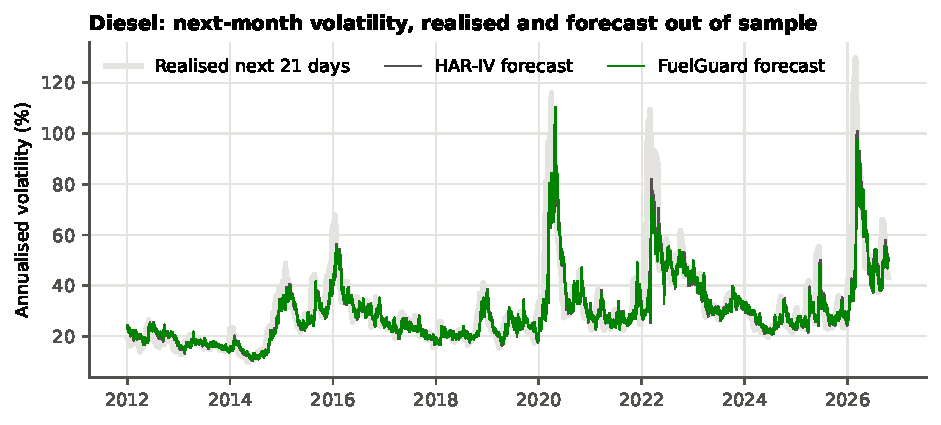
\includegraphics[width=\textwidth]{v2_fig_diesel_forecast.pdf}
\caption{Diesel: realised volatility over the next 21 trading days (grey) and two out-of-sample forecasts
made at the start of the window, 2012--2026.}
\label{fig:diesel}
\end{figure}
